\documentclass{article}
\usepackage{amsrefs}
\usepackage{amssymb}
\usepackage{amsmath}
\usepackage{amsthm}
\usepackage{graphicx}

\newtheorem*{voorbeeld}{Voorbeeld} \newtheorem*{eigenschap}{Eigenschap}

\title{Bepaalde integralen}
\date { }

\begin{document}

\maketitle \noindent

\noindent Voor een functie $f$ continu en positief op een interval $I$ en $a$, $b$ binnen $I$ met $a<b$ noteren we $\int^b_a f(x)dx$ voor de oppervlakte van het vlakdeel begrensd door de $x$-as, de grafiek van $f$ en de verticale rechten $x=a$ en $y=b$.
(Je ziet die oppervlakte gearceerd in volgende figuur.)

\begin{figure}[h]
\begin{center}
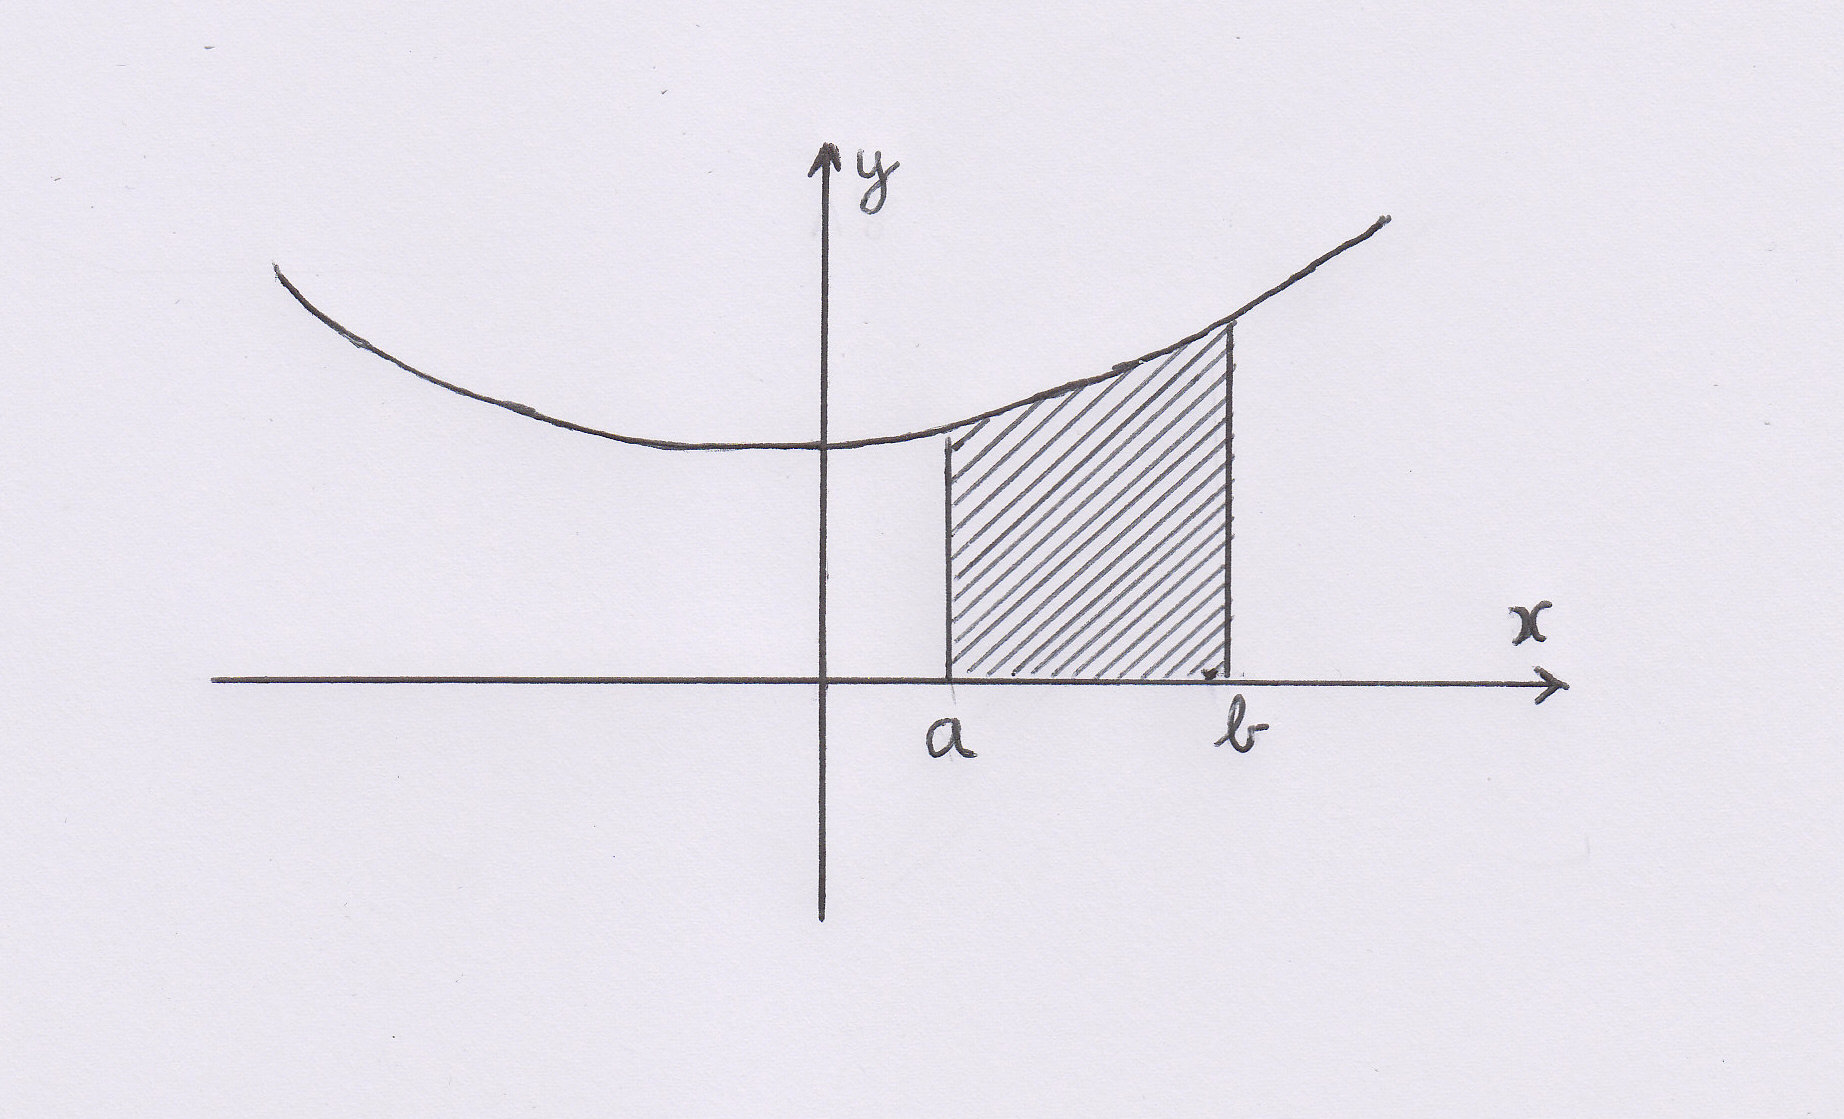
\includegraphics[height=5 cm]{integraal1.JPG}
\end{center}
\end{figure}

\noindent Algemener, als $f$ continu is op een interval $I$ en $a$, $b$ binnen $I$ met $a<b$ dan is $\int ^b_a f(x)dx$ gedefinieerd als de som van de oppervlakten tussen de $x$-as en de grafiek waar de functie $f$ positief is minus de som van de oppervlakten tussen de $x$-as en de grafiek waar de functie $f$ negatief is.
Een + op de volgende figuur duidt een oppervlakte aan die positief meetelt en een - duidt een oppervlakte aan die negatief meetelt.\\

\begin{figure}[h]
\begin{center}
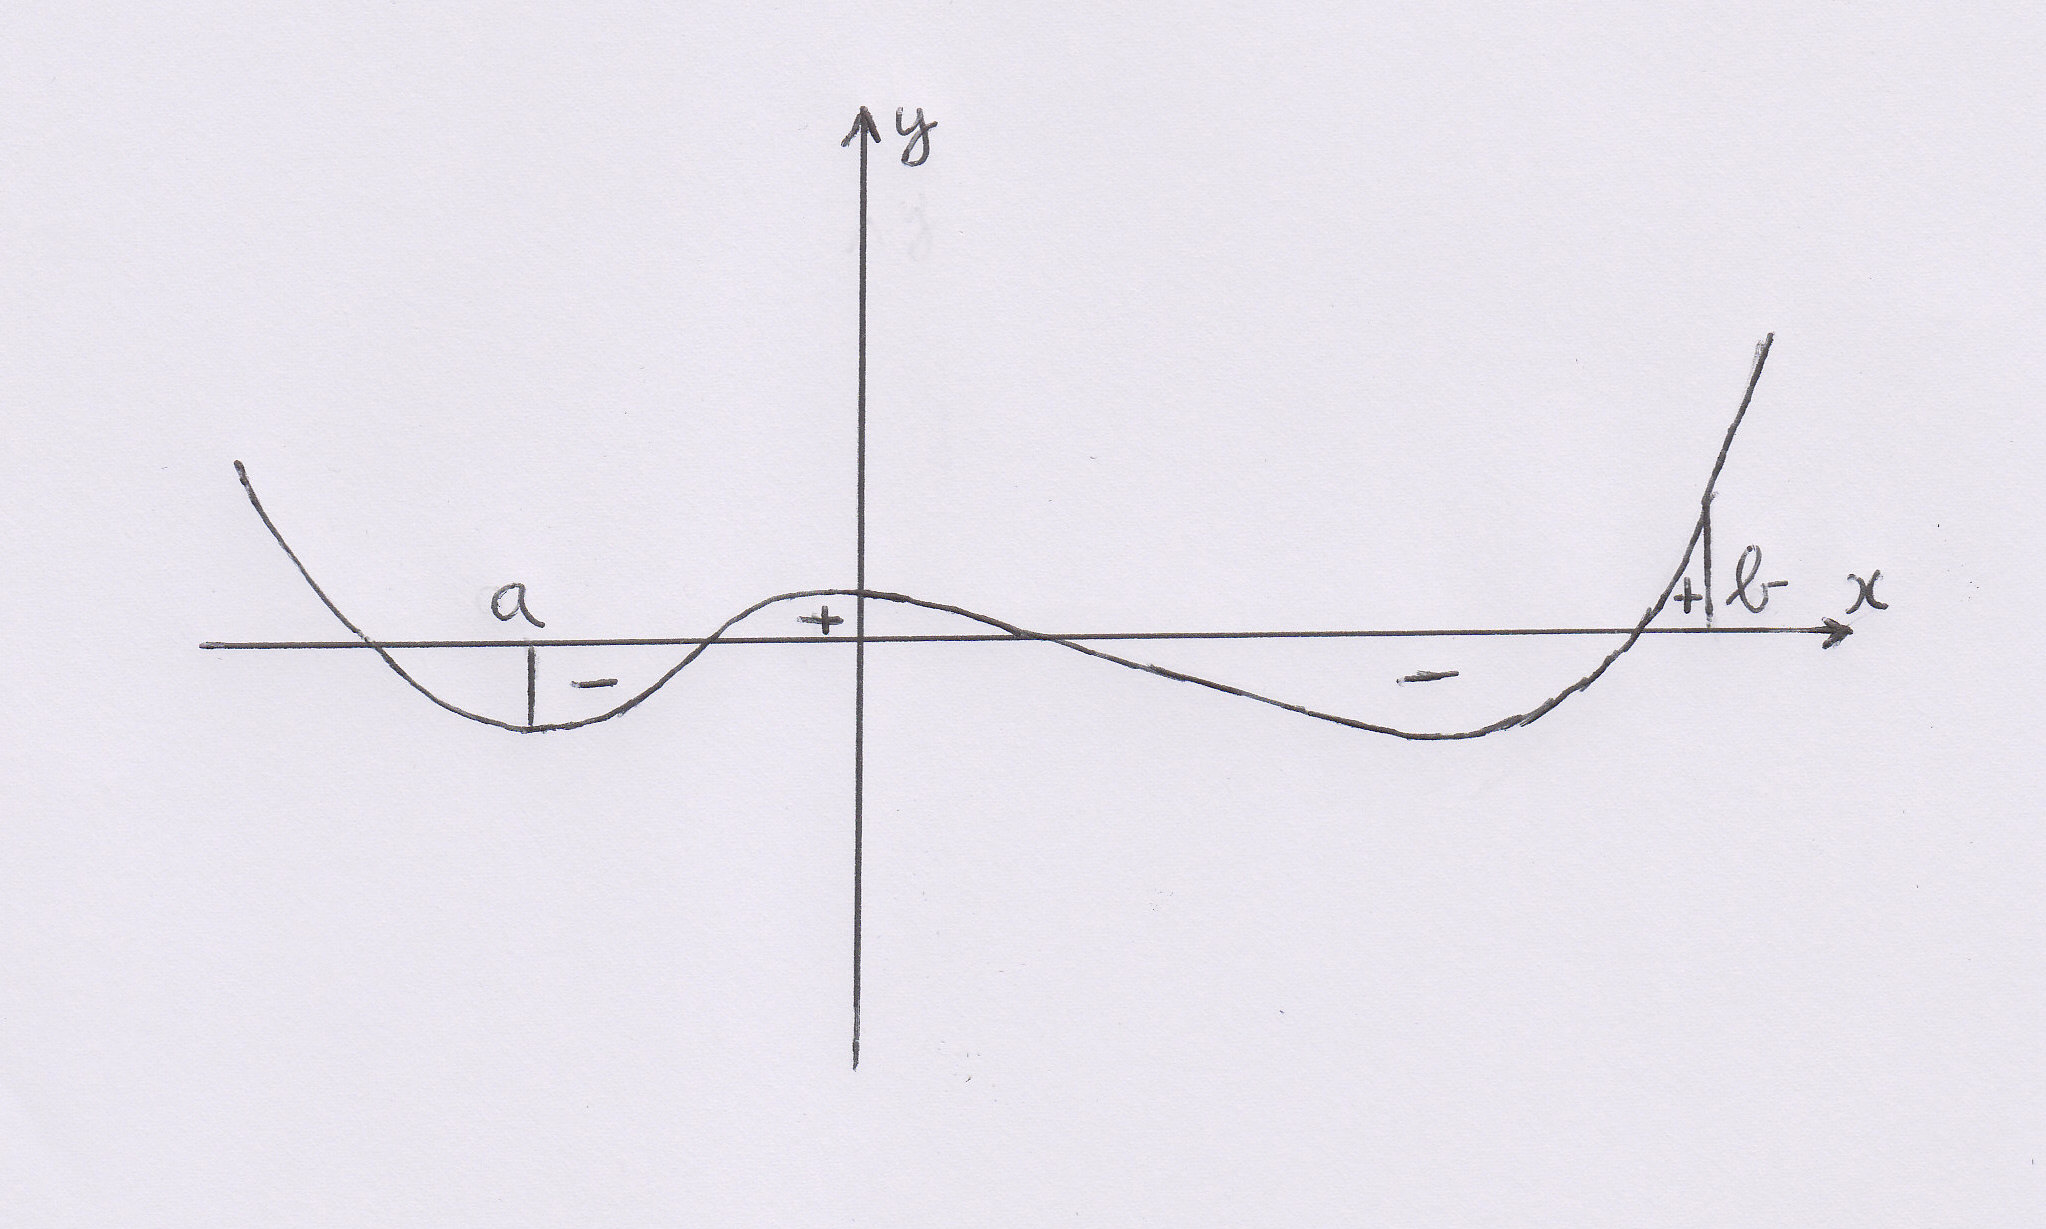
\includegraphics[height=5 cm]{integraal2.JPG}
\end{center}
\end{figure}

\noindent Nog algemener, als $f$ continu is op een interval $I$ en $a$ en $b$ binnen $I$ dan is $\int ^b_a f(x)dx$

\hspace{1cm} reeds gedefinieerd als $a<b$

\hspace{1cm} $-\int^a_b f(x)dx$ als $a>b$

\hspace{1cm} 0 als $a=b$.\\

\noindent Je noemt $\int^b_a f(x)dx$ de bepaalde integraal van de functie $f$ van $a$ naar $b$.\\

\noindent Dank zij de volgende eigenschap kun je bepaalde integralen uitrekenen door middel van onbepaalde integralen.

\begin{eigenschap} Als $f$ een continue functie is op een interval $I$ en $F$ is een primitieve functie van $f$ dan geldt voor elementen $a$ en $b$ van $I$ dat\\
$\boxed { \int^b_a f(x)dx = F(b)-F(a) }$
\end{eigenschap}

\noindent Vorige eigenschap is een gevolg van de belangrijke stelling van Newton-Leibnitz die volgend verband geeft tussen afgeleiden en bepaalde integralen.

\begin{eigenschap}
Als $f$ een functie is continu op een interval $I$ en $a$ is een element van $I$ dan voldoet de functie $F(x) = \int^x_a f(t)dt$ aan $DF(x)=f(x)$ voor alle $x$ in $I$.
\end{eigenschap}

\noindent Deze stelling van Newton-Leibnitz wordt aan de hand van een filmpje getoond in een voorbeeld.

In het filmpje wordt de functie met voorschrift $f(x)=x$ gebruikt. De bijbehorende functie $F(x)$ wordt nu $O(x)$ genoteerd (misschien toch beter met $F(x)$ noteren) en is dus gegeven door de formule rechts bovenaan ($O(x)=\int ^x_0 tdt$).
Voor de gegeven functie $f(x)=x$ is dit de oppervlakte getekend rechts bovenaan.

De drie volgende tekeningen is de situatie voor een aantal waarden van $x$. Als je $x$ opeenvolgend $1$; $2$ en $\frac {1}{2}$ neemt dan bekom je telkens links de bijbehorende oppervlakte die elementair uit te rekenen is (oppervlakte van een driehoek). Rechts staat dan de berekening van die oppervlakte en dat geeft aanleiding tot een punt van de grafiek van die functie $O(x)$. De linkse tekening zijn dus steeds nieuwe tekeningen en de rechtse tekening is een punt meer van de grafiek van $O(x)$.

Op de volgende bladzijde staat dan de berekening voor een willekeurige $x$ , krijg je daardoor het voorschrift van de volledige functie $O(x)$ en de grafiek ervan.

Op de volgende lijn staat dan rechts de afgeleide van die functie $O(x)$ berekend en als je van die afgeleide dan links de grafiek tekent krijg je terug $f(x)=x$, de functie waarmee je startte.

De tekst onderaan geeft terug de formulering van de stelling van Newton-Leibnitz en voor welke functie dat in het filmpje geïllustreerd is.

In de SPOC was het de bedoeling dit zonder bijkomende woorden of tekst te maken, misschien is het in de MOOC toch beter om er tekst en/of geluid bij te plaatsen.

Het is gewoon een idee om een fundamentele stelling uit de wiskunde door middel van een eenvoudig voorbeeld te illustreren. 

\end{document}